\section{Framework}

\subsection{Gestion des fichiers}

La solution choisie pour la gestion des fichiers est de créer un dépendance entre le Framework et l'EJB qui gère les connections à la base de données utilisateur.\\

\paragraph*{Sélection de fichier}

Pour la sélection de fichier, on propose d'utiliser un navigateur de fichier d'un utilisateur. Ce navigateur apparait en pop-up pour gêner au minimum la navigation sur le site web. L'outil retourne un objet File lorsque l'utilisateur sélectionne un fichier. C'est à partir de ce type d'objet que les modules doivent travailler.\\

\paragraph*{Sauvegarde de fichier}

La sauvegarde de fichier se fera à la racine du répertoire associé à l'utilisateur sous la forme "Nom su module"+"date de création du fichier"+"extension". Pour utiliser ce service il suffit de créer une instance de la classe FilesManage. Avec cette instance, appeler la méthode saveFile en lui passant en paramètre les informations nécessaire à la création du fichier. Cette méthode se charge de créer le fichier et de le sauvegarder dans la base de données.\\

\subsection{Gestion des taches}

Pour la gestion des taches, on a créé un singleton TaskManager. Cette classe contient des map ayant pour clef un utilisateur et en valeur les taches lancée par cet utilisateur. Elle contient aussi une instance de ExecutorService, qui permet de constituer un pool de thread. Un pool de thread gère un ensemble de threads travailleurs.Il est étroitement lié à une file contenant des tâches en attente . La vie des thread travailleurs est simple : demander la tâche suivante dans la file, l'exécuter et revenir attendre une autre tâche. Dans notre gestionnaire le nombre de thread travailleurs est fixé dynamiquement en fonction du nombre de processeurs logique sur la machine où est installé l'application.\\
De plus il y a deux autres classes crées : \\
\begin{itemize}
\item une interface Task qui doit être implémenté par le module
\item une classe TaskLauncher qui implémente Runnable et étant Thread
\end{itemize}
Pour lancer une tache il faut :
\begin{verbatim}
TaskManager taskManager = TaskManager.getInstance();
taskManager.addTask(new Task(),utilisateur);
\end{verbatim}
Le gestionnaire propose aussi cd fournir une liste de tache par utilisateur ainsi que leur état. Il propose aussi je supprimer ces taches.\\

\subsection{Gestion des pages web}

Pour développer les pages web nous utilisons Java server faces (JSF) ainsi que le framework RichFaces prenant proposant de multiples fonctionnalités AJAX.  Java Server Faces est un framework de développement applications Web en Java permettant de respecter le modèle d’architecture MVC et basé sur des composants côté présentation.  JSF permet :\\
\begin{itemize}
\item une séparation de la couche présentation des autres couches (MVC)
\item un mapping entre l’HTML et l’objet
\item un ensemble de composants riches et réutilisables
\item une liaison simple entre les actions côté client de l'utilisateur (event listener) et le code Java côté serveur
\item Création de nouveaux composants graphiques
\end{itemize}
Richfaces est produit par JBoss (appartenant à redhat), et est une librairie commerciale de composants JSF.
\begin{figure}[position]
   \caption{Schéma de fornctionnement de JSF + RichFaces +AJAX }
   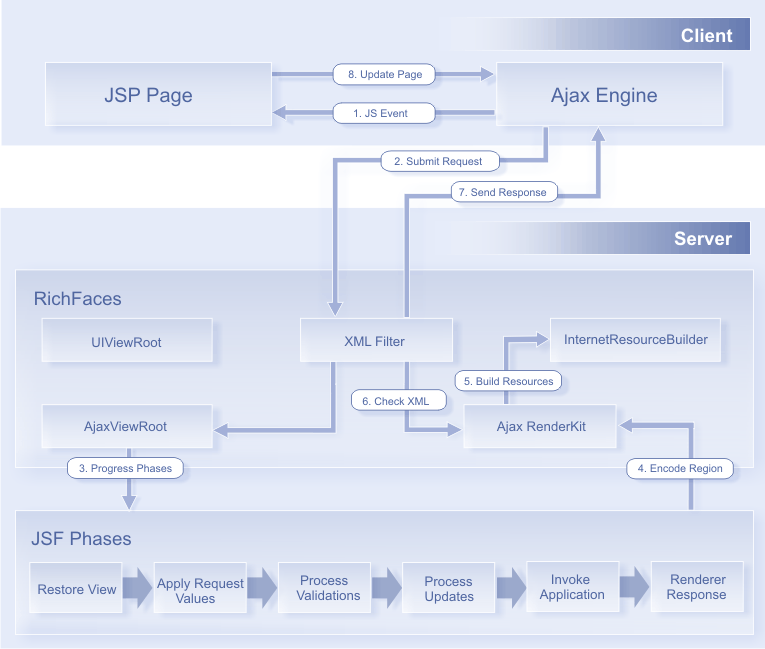
\includegraphics[scale=1]{a4jsfPhases.png} 
\end{figure}

Nous proposons différent encart au développeur de module, un pour le module proprement dit et un pour le menu de son module. Nous utilisons la propriété de JSF permettant de créer nos propres composants graphiques, ainsi on crée trois nouvelles balises :\\
\begin{itemize}
\item \textit{<mbui:menu>} dans laquelle on met le menu du module
\item \textit{<mbui:optionsPanel>} dans laquelle on met les options du module
\item \textit{<mbui:modSpace>} dans laquelle on met le module même
\end{itemize} 